\nonstopmode
\documentclass[10pt, a4paper]{article}
%\usepackage{subfig}

\parindent=20pt
\parskip=8pt
\usepackage[width=15.5cm, left=3cm, top=2.5cm, height= 24.5cm]{geometry}
\usepackage[english]{babel}
\usepackage[utf8]{inputenc}
\usepackage{fancyhdr}
\usepackage{multirow}
\usepackage{rotating}
\usepackage{tabto}
\usepackage{indentfirst}
\usepackage{latexsym}
\usepackage{gnuplottex}
\usepackage{epsfig}
\usepackage{lastpage}
\usepackage{amsfonts}
\usepackage{listings}
\usepackage[export]{adjustbox}
\usepackage{pdfpages}
\usepackage{float}
\usepackage{color}
\usepackage{amssymb}
\usepackage{caratula}


%fancyhdr 
\graphicspath{{imgs/}}
\setlength{\parindent}{0pt}
\pagestyle{fancy}
\thispagestyle{fancy}
\addtolength{\headheight}{1pt}
\lhead{Sistemas Operativos}
\rhead{TP1}
\cfoot{\thepage /\pageref{LastPage}}
\renewcommand{\footrulewidth}{0.4pt}
\renewcommand{\thesubsubsection}{\thesubsection.\alph{subsubsection}}


\newenvironment{changemargin}[2]{%
\list{}{\rightmargin#2\leftmargin#1
\parsep=0pt\topsep=0pt\partopsep=0pt}
\item[]}
{\endlist}

\newenvironment{indentmore}{\begin{changemargin}{1cm}{0cm}}{\end{changemargin}}

\author{Sistemas Operativos, DC, UBA.}
\date{}
\title{}

\begin{document}
%Caratula
	\materia{Sistemas Operativos} % obligatorio
	\submateria{Segundo Cuatrimestre de 2015} % opcional
	\titulo{Trabajo practico 1} % obligatorio
	
	
	\integrante{Integrante Ignacio Rodriguez}{797/13}{igna\_nacho286@hotmail.com} % obligatorio 
	\integrante{Integrante Nicolás Mastropasqua}{828/13}{me.nicolas7@gmail.com} % obligatorio 
	\integrante{Integrante Uriel Fadel}{104/14}{urielfadel@gmail.com} % obligatorio 
	
	
	\maketitle
	% compilar 2 veces para actualizar las referencias
	\tableofcontents
	
	\pagebreak

\section{Ejercicio 1:}



\subsection{Enunciado:}
Programar un tipo de tarea TaskConsola, que simulará una tarea interactiva.
La tarea debe realizar n llamadas bloqueantes, cada una de una duración al azar 1 entre bmin
y bmax (inclusive). La tarea debe recibir tres parámetros: n, bmin y bmax (en ese orden)
que serán interpretados como los tres elementos del vector de enteros que recibe la función.
Explique la implementación realizada y grafique un lote que utilice el nuevo tipo de tarea.

\subsection{Resolución:}
Tarea Consola: Esta tarea recibe tres parámetros: n, bmin y bmax. A partir de esto genera n llamadas bloqueantes con duración al azar(entre bmin y bmax).

Para ello, hacemos un ciclo cuya duración esta indicada por el primer elemento del vector de parametros(n).
En el cuerpo del ciclo, creamos un numero pseudo-aleatorio usando la función \textbf{rand()} y llamamos a \textbf{uso\_IO} con el mismo.
Por defecto, el numero devuelto se encuentra en el rango $[0,rand\_MAX]$. Para que quede definido en $[bmin,bmax]$ basta con lo siguiente:

Sea $rango = bmax - bmin + 1 $

$0$ \hspace{6mm}$\leq$  \hspace{5mm}\textbf{rand()} mod $rango \ < rango = bmax - bmin +1$ 

$bmin\leq$ \hspace{4mm} \textbf{rand()} mod $rango\ + \ bmin \ <  bmax \ - \ bmin \ +1 \ + \ bmin \ = \ bmax \ +1 \leq bmax$

Además \textbf{rand()} generará siempre la misma sucesión de números pseudo-aleatorios en cada nueva ejecución.

Exactamente esta operatoria es la que se hace en el codigo.
\subsection{Gráficos:}

A continuación se muestra un gráfico representando la ejecución de un lote de cuatro tareas: Las de ID cero y uno  del tipo consola, la de ID 2 del tipo \textbf{uso\_cpu} y la ultima del tipo \textbf{uso\_IO}. Todas son manejadas por un scheduler \textit{FCFS(First Come First Served)}. Todas se van incorporando al scheduler con 2 clocks de diferencia.
Notese que, por ejemplo, la primer tarea fue corrida con una duración de 5 clocks(+1) y un rango de $[2,7]$. Se pueden identificar las 5 llamadas, de duración 2,5,3,6,2 en esa secuencia.
\begin{figure}[H]
  	\centering
   	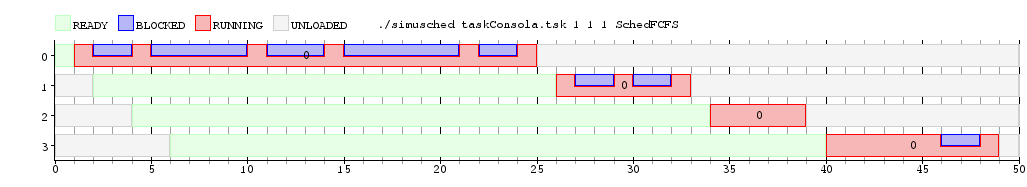
\includegraphics[width=1\textwidth]
   	 {imgs/ej1.png}
	\caption{FCFS con dos TaskConsola, una TaskCPU y otra TaskIO}
\end{figure}


\section{Ejercicio 2:}

\subsection{Enunciado:}Rolando, uno de los investigadores del departamento, utiliza su computadora
para correr un algoritmo muy complejo que hace un uso intensivo de la CPU por 100 ciclos
y no utiliza ninguna llamada bloqueante. Mientras corre su algoritmo suele poner su canción preferida y luego navegar por internet (estas tareas realizan 20 y 25 llamadas bloqueantes respectivamente con una duración variable entre 2 y 4 ciclos).
Escribir el lote de tareas que simule la situación de Rolando. Ejecutar y graficar la simulación usando el algoritmo FCFS para 1 y 2 núcleos con un cambio de contexto de 4 ciclos. Calcular la latencia de cada tarea en los dos gráficos. Explicar qué desventaja tendría Rolando si debe mantener este algoritmo de scheduling y sólo tiene disponible una computadora con un núcleo, 
\subsection{Resolución:}

Para simular esta situación con el scheduler \textbf{FCFS},se armo un lote de tareas como se muestra en la tabla de abajo. Decidimos dejar un tiempo prudencial entre cada una de ellas para cumplir, de cierta forma, con la serializacion que ,entendemos, describe en el problema(Rolando corre su algoritmo, pone su canción y después navega por internet).
El mismo lote se utilizo para ambos casos.
\begin{center}
\begin{tabular}{| l | l | l | l |}
    \hline
    Tarea & TiempoLlegada \\ \hline
    TaskCPU &	0 \\ \hline 
    TaskConsola & 20 \\ \hline
     TaskConsola & 40 \\ \hline

\end{tabular}
\end{center}
\begin{flushleft}
\textbf{Primer Caso:}\\
\end{flushleft}	
A continuación se muestra la tabla que se obtiene de simular la situación planteada para un solo núcleo. Los resultados se condicen con el gráfico de la figura 2
\begin{center}
\begin{tabular}{| l | l | l | l |}
    \hline
    Tarea & Latencia(en ciclos)\\ \hline
   TaskCPU &	4 \\ \hline 
   TaskConsola & 89 \\ \hline
TaskConsola & 150 \\ \hline
\end{tabular}
\end{center}

\begin{center}
  \textit{Los valores exactos fueron extraídos desde la ejecución en consola}
\end{center}

\begin{flushleft}
\textbf{Segundo Caso:}\\
\end{flushleft}

A continuación se muestra la tabla que se obtiene de simular la situación planteada para dos núcleos. Los resultados se condicen con el gráfico de la figura 3

\begin{center}
\begin{tabular}{| l | l | l | l |}
    \hline
    Tarea & Latencia(en ciclos)\\ \hline
   TaskCPU &	4 \\ \hline 
   TaskConsola & 4 \\ \hline
TaskConsola & 65 \\ \hline
\end{tabular}
\end{center}
\begin{center}
  \textit{Los valores exactos fueron extraídos desde la ejecución en consola}
\end{center}

\subsection{Gráficos:}

\begin{figure}[H]
  	\centering
   	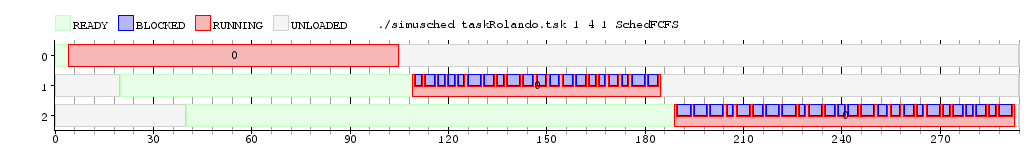
\includegraphics[width=1\textwidth]
   	 {imgs/Rolando1Core.png}
	\caption{1 core}
\end{figure}

\begin{figure}[H]
  	\centering
   	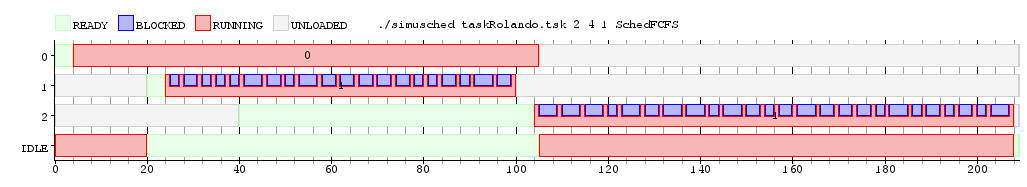
\includegraphics[width=1\textwidth]
   	 {imgs/Rolando2Core.png}
	\caption{2 core}
\end{figure}


En este escenario, se puede observar que la duración del lote de tareas en el caso de un solo núcleo(figura 2) finaliza después de los 290 ciclos, mientras que con dos(figura 3), no supera los 210. 
Esto se debe a la ganancia en la latencia del segundo caso con respecto al primero. Como se puede ver en el gráfico, y en los cálculos previos, la tarea 1 llega en el ciclo 20  y solo pasa 4 en estado ready pues luego es "recibida" por el segundo núcleo, que hasta el momento se encontraba ejecutando la tarea IDLE(desde 0 a 20 ciclos, como se puede apreciar)
Esta situación seria imposible en el caso 1, ya que la tarea 1 debe esperar(por razones de la implementación FCFS y por la ausencia de un segundo núcleo) a que la tareaCPU(ID = 0) llegue a su fin(como se puede ver al cabo de los 105 ciclos). \\

Por estas razones es que ,también, la ultima tarea(ID = 2) reduce el tiempo de latencia, aproximadamente acla mitad, en el caso 2, ya que ahora a los 105 ciclos, el primer núcleo se libera de la tareaCPU y luego del context switch de 4 ciclos, se comienza a ejecutar.
Es importante marcar que las tareas que simulan la reproducción de una canción y la navegación, realizan una cantidad de llamadas bloqueantes de duración entre 2 y 4 ciclos, durante las cuales el flujo de ejecución queda estático, es decir es tiempo que el cpu "desperdicia" , a diferencia de Round Robin, donde se cambiaría inmediatamente a otro proceso.

Notese que hay un ciclo adicional por tarea, siendo este la llamada a la syscall exit().
\section{Ejercicio 3:}

\subsection{Enunciado:}

Programar un tipo de tarea TaskBatch que reciba dos parámetros: total cpu y
cant bloqueos. Una tarea de este tipo deberá realizar cant bloqueos llamadas bloqueantes, en
momentos elegidos pseudo aleatoriamente. En cada tal ocasión, la tarea deberá permanecer
bloqueada durante exactamente un (1) ciclo de reloj. El tiempo de CPU total que utilice una
tarea TaskBatch deberá ser de total cpu ciclos de reloj (incluyendo el tiempo utilizado para
lanzar las llamadas bloqueantes; no así el tiempo en que la tarea permanezca bloqueada).
Explique la implementación realizada y grafique un lote que utilice 3 tareas TaskBatch con
parámetros diferentes y que corra con el scheduler FCFS.
\subsection{Gráficos:}

El siguiente lote de tareas es el utilizado para graficar como funciona la tarea taskBatch.

\begin{center}
\begin{tabular}{| l | l | l | l |}
    \hline
   Tarea & TotalCpu & CantBloqueos \\ \hline
  TaskBatch & 20 & 2 \\ \hline
TaskBatch & 60 & 9 \\ \hline
TaskBatch & 22 & 5 \\ \hline

\end{tabular}
\end{center}




\begin{figure}[H]
  	\centering
   	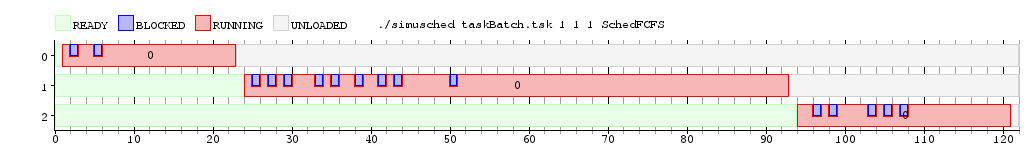
\includegraphics[width=1\textwidth]
   	 {imgs/Batch.png}
	\caption{}
\end{figure}



\subsection{Resolución:}

La forma de solucionar el ejercicio, basándonos en que el tiempo total que el proceso necesita de CPU + la cantidad de ciclos que se bloquean (ya que necesitan un ciclo de procesador) + 1 ciclo de return, es el primer parámetro, y el segundo parámetro es la cantidad de llamadas bloqueantes.

 Entonces la forma en la que está pensado es: Armamos un vector en el que lo llenamos de la forma  $[1,2,3,4,5,..,n]$, con $n$ siendo la cantidad de ciclos que se necesitan de CPU. Luego usamos una función de la std que hace una permutación aleatoria de un array. Como ahí ya están los números de una forma aleatoria, agarramos los m primeros valores, con m siendo la cantidad de llamadas bloqueantes de 1 ciclo. 
De esa forma tendríamos m valores, que serían las instancias de tiempo en el que el proceso se va a bloquear por 1 ciclo. Creamos un array, inicializado  todo en 0, y luego recorremos los primeros m valores del vector (las instancias en la que vamos a bloquear el proceso) y  por cada uno de ellos indexamos el array con su valor, colocando  un 1 en dicha posición.

 Luego vamos a recorrer este array, que tiene un 0 en las posiciones (que corresponden a las instancias de tiempo) que se va a correr el CPU, y un 1 en las que se va a bloquear. Y al recorrerlo, si es 0 llamamos a la función uso$\_$CPU(1) y si es 1, uso$\_$IO(1).   

\section{Ejercicio 4:}
\subsection{Enunciado:}
Completar la implementación del scheduler Round-Robin implementando los
métodos de la clase SchedRR en los archivos sched rr.cpp y sched rr.h. La implementación
recibe como primer parámetro la cantidad de núcleos y a continuación los valores de sus
respectivos quantums. Debe utilizar una única cola global, permitiendo así la migración de procesos entre núcleos.
\subsection{Resolución:}
Para la implementación del Round Robin se usa una cola y dos arreglos de enteros. En la cola se van a guardar por orden a cual es la próxima a correr todas las tareas que no estén corriendo. En uno de los arreglos, que llamamos quantum, se van a guardar  los quantums de cada core, esto se hace en el momento de la inicialización del round robin. En el otro arreglo, llamado contadores, que en un principio esta inicializado en cero.

Luego, en un principio el programa se va a fijar si la cola esta vacía hace que se corra la tarea idle, si no, se desencola la primera tarea y se la corre. En cada tick se va a incrementar el contador del core respectivo, y se va a ver si el contador llego al quantum del core, en caso de que no pase esto se sigue corriendo la tarea, pero si ya se corrió todo el quantum, se pone el contador en 0, y se va a ver si la cola esta vacía. En caso de estar vacía se vuelve a correr la tarea que estaba corriendo, si no, se desencola la primer tarea y se encola la tarea que estaba corriendo, y se pone a correr la tarea desencolada.

Cuando una tarea se bloquea o termina simplemente se fija si la cola esta vacía o no, si esta vacía se corre la tarea idle, si no se corre la primer tarea de la cola. Cuando se desbloquea una tarea se encola en la cola de vuelta.

\section{Ejercicio 5:}

\subsection{Enunciado:}
Diseñe un lote con 3 tareas de tipo TaskCPU de 50 ciclos y 2 de tipo TaskConsola con 5 llamadas bloqueantes de 3 ciclos de duración cada una. Ejecutar y graficar la simulación utilizando el scheduler Round-Robin con quantum 2, 10 y 50. Con un cambio de contexto de 2 ciclos y un sólo núcleo calcular la latencia, el waiting time y el tiempo total de ejecución de las cinco tareas para cada quantum. ¿En cuál es mejor cada uno? ¿Por qué ocurre esto?

\subsection{Resolución:}

Primero, hacemos algunas aclaraciones pertinentes.En el  lote implementado, todas las tareas llegan al sistema en el ciclo inicial.
En las tareas del tipo TaskConsola, el waiting time (por definición los ciclos que pasa la tarea en estado \textit{ready}), no incluye los ciclos que se encuentra en estado bloqueada.
Para el running time , consideramos la cantidad de ciclos que le toma a la tarea ejecutarse, es decir desde que recibe por primera vez el cpu, hasta que finaliza por completo.

\begin{flushleft}
\textbf{Primer Caso: Quantum 2}\\
\end{flushleft}


A continuación se muestra la tabla que se obtiene de simular la situación planteada. Los resultados se condicen con el gráfico de la figura 5	
\begin{center}
\begin{tabular}{| l | l | l | l |}
    \hline
    IDtarea & Latencia(en ciclos)& Waiting time & Running time\\ \hline
    Tarea0 & 	2 	&	288	&  	338 \\ \hline
    Tarea1 &	6	&	292	& 	337 \\ \hline
    Tarea2 &	10	&	296	&	346 \\ \hline
    Tarea3 &	14	&	79	& 	92 \\ \hline
    Tarea4 &	17	&	82	&	92 \\ \hline

\end{tabular}
\end{center}
\begin{center}
  \textit{Los valores exactos fueron extraídos desde la ejecución en consola}
\end{center}


\begin{flushleft}
\textbf{Segundo Caso: Quantum 10}\\
\end{flushleft}


A continuación se muestra la tabla que se obtiene de simular la situación planteada. Los resultados se condicen con el gráfico de la figura 6	
\begin{center}
\begin{tabular}{| l | l | l | l |}
    \hline
    IDtarea & Latencia(en ciclos)& Waiting time & Running time\\ \hline
    Tarea0 & 	2 	&	167	&  	212 \\ \hline
    Tarea1 &	14	&	170	& 	203 \\ \hline
    Tarea2 &	26	&	173	&	194 \\ \hline
    Tarea3 &	38	&	206	& 	185 \\ \hline
    Tarea4 &	41	&	209	&	185 \\ \hline

\end{tabular}
\end{center}
\begin{center}
  \textit{Los valores exactos fueron extraídos desde la ejecución en consola}
\end{center}


\begin{flushleft}
\textbf{Segundo Caso: Quantum 50}\\
\end{flushleft}

A continuación se muestra la tabla que se obtiene de simular la situación planteada. Los resultados se condicen con el gráfico de la figura 7
\begin{center}
\begin{tabular}{| l | l | l | l |}
    \hline
    IDtarea & Latencia(en ciclos)& Waiting time & Running time\\ \hline
    Tarea0 & 	2 	&	114	&  	164 \\ \hline
    Tarea1 &	54	&	117	& 	115 \\ \hline
    Tarea2 &	106	&	121	&	66 \\ \hline
    Tarea3 &	158	&	178	& 	40 \\ \hline
    Tarea4 &	161	&	181	&	41 \\ \hline

\end{tabular}
\end{center}
\begin{center}
  \textit{Los valores exactos fueron extraídos desde la ejecución en consola}
\end{center}

\subsection{Gráficos:}
\begin{figure}[H]
  	\centering
   	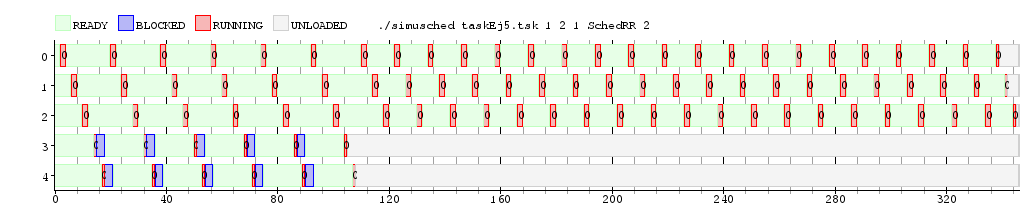
\includegraphics[width=1\textwidth]
   	 {imgs/quantum2.png}
	\caption{Quantum = 2}
\end{figure}


\begin{figure}[H]
  	\centering
   	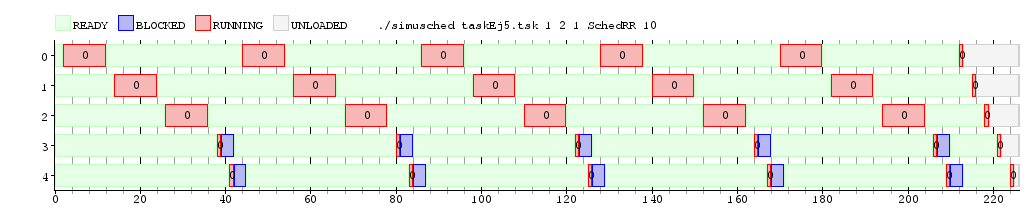
\includegraphics[width=1\textwidth]
   	 {imgs/quantum10.png}
	\caption{Quantum = 10}
\end{figure}



\begin{figure}[H]
  	\centering
   	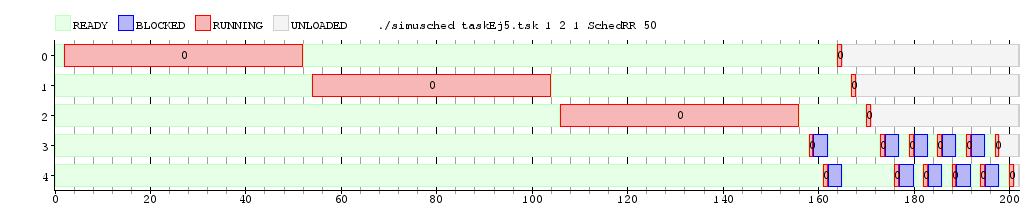
\includegraphics[width=1\textwidth]
   	 {imgs/quantum50.png}
	\caption{Quantum = 50}
\end{figure}
	

\begin{flushleft}
\textbf{¿En cual caso es mejor cada uno de los parámetros medidos? ¿Por que ocurre esto?}\\

\end{flushleft}


Los cálculos, basados en los datos que arroja el simulador y respaldados por lo que se observa en el gráfico, nos permitirán sacar conclusiones sobre los aspectos medidos: Latencia, Waiting Time y Running Time.
En el caso de la latencia, se ve que aumenta conforme lo hace el quantum. Esto se debe a que , asumiendo que todas las tareas llegan en el instante inicial como lo hacen en los graficos, las mismas deben esperar rondas de mayor tiempo para poder comenzar a ejecutar. Tambien se podría observar, por la misma razon, que si el costo del cambio de tareas aumentase, la latencia tambien lo hará.

Sin embargo, el waiting time decrece ,para todos los procesos ,del tipo TaskCPU, si el Quantum lo hace.
Si se define el overhead producido por los context switch(son tiempos de procesamiento "desperdiciado") como: \\

\begin{center}
\textbf{context switch overhead} = $\frac{C}{(Q+C)}$
\end{center}

Donde $Q$ = quantum y $C$ = costo del context switch

Podemos ver que si  aumentamos $Q$, con el $C$, estaremos disminuyendo el tiempo que se "desperdicia" en hacer los cambios entre tareas.
Además, como otra consecuencia, se aumentará el tiempo que los procesos tienen a su disposición el cpu antes de ser desalojados,pero ,a su vez, incrementando el waiting time entre ronda. En este caso, la combinación  resulta favorable para las tareas TaskCpu, no así para las tareas Consola, que para poder ejecutar las cinco llamadas, deberán esperar al menos 5 rondas, cuya duración aumento con respecto a las de Quantum 2.

Cuando subimos el quantum a 50, observamos una situación particular. Cada tarea TaskCpu puede terminar en una ronda, por lo tanto se reducen drásticamente la cantidad de ciclos desperdiciados en los cambios de contexto, al mismo tiempo que se reduce el Waiting time, en detrimento de la latencia, como se explico anteriormente. Este escenario genera, entonces, un tiempo de respuesta ,para los procesos que no son atendidos de inmediato(como las tarea 3 y 4), mucho mayor. Esta penalidad podria no ser deseable en situaciones donde se corren tareas interactivas.
Se ve también que la situación para las tareas Consola mejora levemente, ya que el waiting time disminuye dado que luego de realizar las dos primeras llamadas, no hay mas taras Consola en la cola del scheduler(como se observa en el gráfico, promediando el ciclo 180), por lo que pueden alternarse entre ellas y finalizar mas rápidamente las llamadas restantes.
En conclusión, las tareas Consola obtuvieron su mejor waiting time con Quantum 2, donde el era lo suficientemente chico como para completar rápidamente sus llamadas, debido a que el tiempo esperado por ronda era menor. Esta situación, pudo verse también con Quantum = 50 sobre el final de la ejecución(por la particularidad que se explico anteriormente). Sin embargo, no fue óptimo porque también sufrieron un notable aumento en la latencia, con respecto al primer escenario.


Como consecuencia de lo anteriormente explicado es que se obtiene un running time óptimo, para estos casos, con Quantum = 50.
Es decir, en este ultimo escenario ,el scheduler tuvo un desempeño similar al de un FCFS(ver figura 8) que, debido a la naturaleza de las tareas elegidas de este caso, minimiza el running time.


\section{Ejercicio 6:}
	
\subsection{Enunciado:}
Grafique el mismo lote de tareas del ejercicio anterior para el scheduler FCFS.
Haciendo referencia a lo que se observa en los gráficos de este ejercicio y el anterior, explique las diferencias entre un scheduler Round-Robin y un FCFS.

\subsection{Gráficos:}


\begin{figure}[H]
  	\centering
   	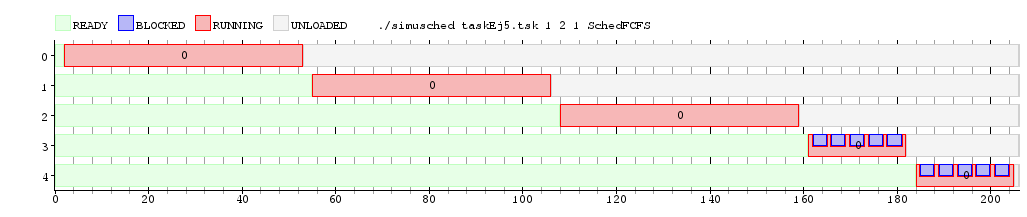
\includegraphics[width=1\textwidth]
   	 {imgs/ej6.png}
	\caption{Ejercicio 5 con FCFS}
\end{figure}
\subsection{Resolución:}

Una de las diferencias importantes entre Round Robin, y First Come First Served, es el tiempo que se pierde entre cada cambio de contexto.
Tiene un beneficio que es el hecho de  que el tiempo en el que un proceso es bloqueado no pierde tiempo de procesamiento, pero sin embargo con 
lo que cuesta un cambio de contexto, y mas cuando los quantums son tan chicos y el cambio de contexto tan grande, se pierde mucho tiempo
cada vez que necesita cambiar de tarea.
Esto se puede ver en el gráfico de quantum 2, ya que tarda tanto tiempo en cambiar el contexto de lo que se tiene de procesador, sin embargo
cuando vamos agrandando los quantums a 10 o 50, y se mantiene el tiempo de cambio de contexto de 2, entonces se aprovecha un poco mas el procesador
y ahí sí le sirve sacárselo en tiempo de bloqueo.

Otra diferencia entre FCFS y Round Robin, es el tiempo de latencia, ya que en el primero no se empezaran los siguientes procesos hasta no haber completado los anteriores, entonces se tarda demasiado en empezar a atenderlos. Sin embargo el waiting time de los primeros procesos es más corto, pero el de los últimos dos es bastante más grande, ya que tienen que esperar a que terminen los primeros procesos, que tardan bastantes ciclos.En el caso mostrado, al no perder tanto tiempo en cambio de contexto y al haber pocos bloques, o de poca duración, hace que el FCFS funcione más rápido porque el tiempo de cambio de contexto es el mismo, y solo se pierde cuando termina cada uno de los procesos (ya que no se les quita el procesador, i.e no hay desalojo). El FCFS tendría más problemas si los bloqueos fuesen de mayor tiempo. Además ,al menos en este caso, como contrapartida, esta política admite una mayor pérdida de paralelismo en comparación con Round Robin.

Pero la mayor diferencia se ve en que el Round Robin, tiene un quantum. Esto quiere decir que a cada proceso se le va a dedicar una cantidad de tiempo, y luego se lo va a desalojar, trayendo al próximo proceso, dándole un quantum, y así un ciclo, hasta que todas  terminen. Además el Round Robin tiene desalojo, al contrario de First Come First Serve, que va a empezar a correr una tarea hasta terminarla.


\section{Ejercicio 7:}

\subsection{Enunciado:}
El scheduler SchedMistery fue creado por docentes investigadores de nuestra
materia y ha sido destacado en la última publicación de ACM - SIGOPS, Operating Systems
Review. Desde entonces, numerosos investigadores de todo el mundo nos han contactado para
pedirnos su código fuente. Sin embargo, su código no aparece en ninguno de los repositorios
de la materia y nadie parece recordar quiénes habían estado detrás de su implementación.
Se les pide experimentar con dicho scheduler (aprovechando que hemos conseguido el códi-
go objeto) y replicar su funcionamiento en SchedNoMistery. Graficar como máximo tres lotes
de tareas utilizados en los experiementos y explicar en cada uno por separado qué características de SchedMistery identificaron con ese lote.


\subsection{Gráficos:}

En el siguiente gráfico observamos,principalmente, que  cada parámetro determina el quantum , en orden, que van a ejecutar los procesos. Esto sugiere tener multiples colas, cada una con la duración indicada en la lista de numeros de entrada. Notar, que además se comporta similar a un Round Robin. La primer ronda será, siempre, de 1 quantum y luego las siguientes seran del tamaño indicado por los parametros, en orden. 
Finalmente, cada vez que una tarea termina de ejecutar el quantum asociado a una cola,avanza a la siguiente. Si esta en la ultima, permanecerá en la misma(a menos que llegue un bloqueo, ver mas adelante).

\begin{figure}[H]
  	\centering
   	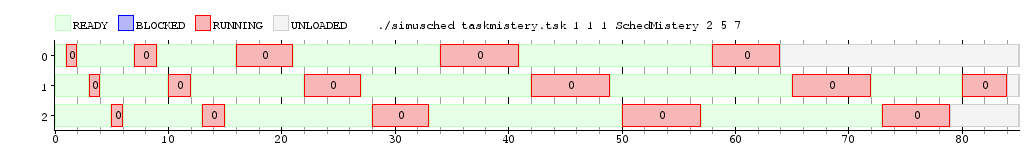
\includegraphics[width=1\textwidth]
   	 {imgs/mistery2.png}
	\caption{}
\end{figure}

En el siguiente grafico observamos lo que ocurre cuando llegan tareas en diferentes tiempos. La de id0 se desaloja al terminar su segunda ronda(la primera con q= 1 y la segunda con q = 2). Luego se ejecutan la id1 y id2, tambien dos rondas hasta terminar aquella con q = 2. Luego se comportan haciendo round robin, y cambiando sus quantums, como se explico arriba.
Esto muestra otra caracteristica. Las tareas se encolan siempre en las primer cola y luego van avanzando a las siguientes. Sin embargo, si en un momento dado llega una nueva tarea, la misma tiene mas prioridad y entonces es ejecutada. Mas aun, cada vez que llegue un nuevo \textbf{tick} el scheduler buscara y ejecutará la tarea que se encuentre en el tope de la primer cola no vacia. Continuará ejecutando las de la misma cola hasta que no haya ninguna (pues las tareas van avanzando a la siguiente). Es decir, siempre vaciará en orden las colas, comenzando desde la de q = 1.
De esta forma, las tareas que van llegando iran alcanzando a las que ya se estaban ejecutando, hasta estar al mismo ``nivel de prioridad'' (si es que no terminan antes o se bloquean)

\begin{figure}[H]
  	\centering
   	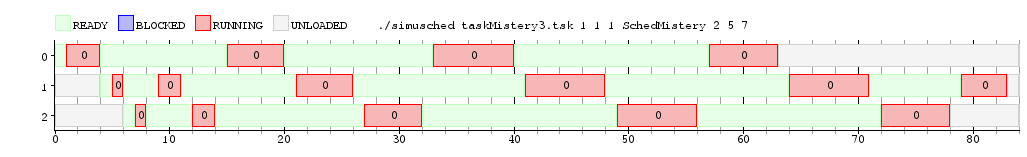
\includegraphics[width=1\textwidth]
   	 {imgs/mistery3.png}
	\caption{}
\end{figure}


Finalmente, acá observamos el comportamiento cuando los procesos se bloquean. Si bien utilizamos varios lotes para darnos cuenta de ello, aca se ve un ejemplo.
Cada vez que una tarea sea bloquea, retrocede una nivel en las colas. Es decir, pasa a la anterior. Si la tarea fuese a bloquearse en cada ronda que le es otorgado el cpu, como en el caso del siguiente gráfico, donde a partir del ciclo 30 hasta el 60  la tarea se bloquea tres veces, una en cada ronda, entonces terminara bajando 3 niveles. 
Siguiendo el ejemplo, vemos que cuando la tarea se bloquea por primera vez, estaba en la cola de q = 7 (aunque no llega a ejecutarlos todos). La tara 0 se encuentra ya en la cola de q = 7.,Al estar la otra bloqueada, se pone a ejecutar. Luego, la tarea 1 vuelve a bloquearse, estando en la cola de q = 5. Ocurré lo mismo que antes y cuando el cpu se le es cedido, vuelve a bloquearse y pasa a la cola de q = 2. Una vez mas, en el ciclo 55 pasa lo mismo y entonces la tarea pasa a la cola de q = 1 (Notar que aunque se siga bloqueando, no prosperará, es decir se quedará siempre en la misma). Finalmente, cuando le vuelve a tocar la ronda, la tarea ejecuta 8 ciclos = ($q_{1}$ + $q_{2}$ +$q_{3}$ = 1 + 2 + 5).   
\begin{figure}[H]
  	\centering
   	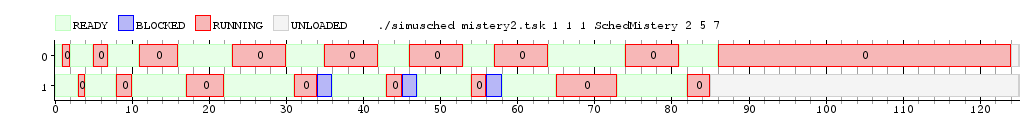
\includegraphics[width=1\textwidth]
   	 {imgs/mistery1.png}
	\caption{}
\end{figure}

\subsection{Resolución:}

Básicamente, el código reune ciertas caracteristicas de la implementacion de Round Robin, junto con la lógica que se explico previamente.
Se tiene un vector de colas, una variale \textbf{corrio} que indica cuantos ticks lleva ejecutando una tarea,  un vector de quantum que tiene la lista de enteros de entrada y otro vector \textbf{colaXtarea} que indica dado el pid de una tarea, en que cola se encuentra.
Es necesario garantizar el invariante de estas estructuras. Cuando llega un tick, si una tarea  termina su quantum , es decir corrio iguala al quantum de la cola en la que esta la tarea, ademas de encolarse en la cola siguiente a la que esta ( a menos que sea la última) se modifica el valor de su posicion en colaXtarea.
Cada vez que llega una tarea, se encola en la primera del vector de colas y ademas se agrega al final de colaXtarea.
Cada vez que se desbloquea una tarea, su posicion en ColaXtarea se decrementa uno y se utiliza este valor para indexar el vector de colas, pusheando la tarea en él.
Si llega un tick y corrio coincide con el quantum de la cola en la que esta la tarea actual, además de preservar los invariantes como se mencionó, se busca la proxima tarea a ejecutar, que será el tope de la primer cola no vacía, y se resetea la variable corrio. Si, en cambio, la tarea ,todavía, no alcanza su quantum, simplemente se aumenta corrio y se  devuelve el mismo pid.
Cuando la tarea termina, o se bloquea, también se busca la proxima a ejectuar de la misma manera. Sin embargo, si no se encuentra ninguna, se seleccionará la idle.

\section{Ejercicio 8:}
	
\subsection{Enunciado:}
Implemente un scheduler Round-Robin que no permita la migración de procesos
entre núcleos (SchedRR2). La asignación de CPU se debe realizar en el momento en que se produce la carga de un proceso (load). El núcleo correspondiente a un nuevo proceso será aquel
con menor cantidad de procesos activos totales (RUNNING + BLOCKED + READY). Explique un escenario real donde la migración de núcleos sea beneficiosa y uno donde no (mencione
específicamente qué métricas de comparación vistas en la materia mejorarían en cada caso).
Diseñe un lote de tareas en nuestro simulador que represente a cada uno de esos escenarios y grafique su resultado para cada implementación. Calcule y compare en cada gráfico las
métrica que mencionó.


\subsection{Gráficos:}
A continuación se mostraran escenarios en los cuales la migración de núcleos resulta favorable y otros en los que no ocurre.

Caso 1: Ambos schedulers corren el siguiente lote de tareas, con el mismo quantum y cantidad de núcleos.

\begin{center}
\begin{tabular}{| l | l | l | l |}
    \hline
    IDtarea &  Tipo & Instante de llegada& Tiempo De Ejecución\\ \hline
    Tarea0 & 	TaskCpu & 0&80 \\ \hline
    Tarea1 &	TaskCpu & 5&5 \\ \hline
    Tarea2 &	TaskCpu & 6&30 \\ \hline
   
\end{tabular}
\end{center}

A continuación se muestra los cálculos,que se desprenden de los gráficos de la figura 12 y 13.

\begin{center}
Figura 12
\end{center}

\begin{center}
\begin{tabular}{| l | l | l | l |}
    \hline
    IDtarea &  Running Time & Waiting time\\ \hline
    Tarea0 & 	87 & 6  \\ \hline
    Tarea1 & 	5 & 1 \\ \hline
    Tarea2 &	39 & 7 \\ \hline
    
   
\end{tabular}
\end{center}
\begin{center}
Throughput = $\frac{3}{88} = 0,034$
\end{center}
\begin{center}
Figura 13
\end{center}

\begin{center}
\begin{tabular}{| l | l | l | l |}
    \hline
    IDtarea &  Running Time & Waiting time \\ \hline
    Tarea0 & 	 136 & 53 \\ \hline
    Tarea1 & 	5 & 1 \\ \hline
    Tarea1 &	84 & 52 \\ \hline
   
\end{tabular}
\end{center}

\begin{center}
Throughput = $\frac{3}{136} = 0,022$
\end{center}

\begin{figure}[H]
  	\centering
   	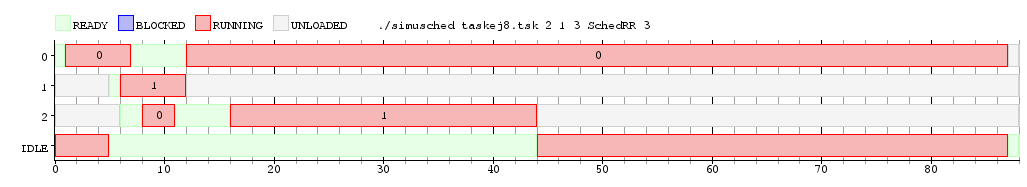
\includegraphics[width=1\textwidth]
   	 {imgs/8Migracion1.png}
	\caption{Situación favorable con migración. Q = 3, N = 2, Tmigracion = 3.}
\end{figure}


\begin{figure}[H]
  	\centering
   	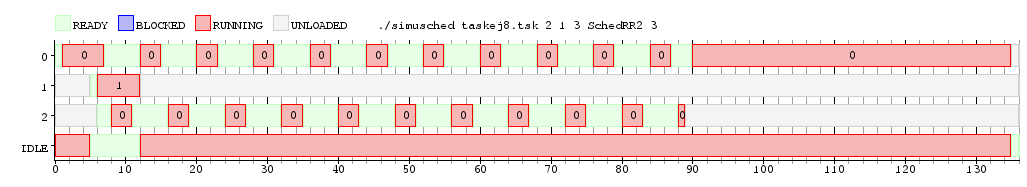
\includegraphics[width=1\textwidth]
   	 {imgs/8NoMigracion1.png}
	\caption{Situación desfavorable sin migración. Q = 3, N=2.}
\end{figure}



Este pequeño ejemplo sirve para ilustrar un caso en el que la migración de procesos resulta en un \textbf{running time} mejor para todos los procesos. 
No solo eso, sino que también reduce el \textbf{waiting time}. La particularidad que produce este comportamiento, es la llegada de una tarea(\textbf{Id1}), de una duración corta, justo antes de que comience a ejecutar la de \textbf{Id2}. Esto le otorgará el núcleo 1 a la misma,
forzando a que la primer tarea(\textbf{Id0}) ceda el suyo(al finalizar el quantum) a la de \textbf{Id2}(ya que la de \textbf{Id1} aun no habrá terminado su quantum y no habrá libera el núcleo). Al finalizar el quantum, la tarea de \textbf{Id2} se desaloja en el core cero, e ingresa la de \textbf{Id0}. Sin embargo, como la tarea de \textbf{Id1} termina pronto, el núcleo 1 quedara disponible inmediatamente para que pueda ser usado por la de \textbf{Id2}.
Como hay migración, la próxima ronda que le sea concedida a la tarea de \textbf{Id2} sera ejecutada en este núcleo(pues el cero esta ocupado con la de \textbf{Id0}). Esta situación, no hubiese
posible de no existir esta cualidad en el scheduler, provocando así que cada tarea quede "fija"  en su núcleo.Este hecho queda evidenciado en la figura 10. 
Como las mas largas fueron adjudicadas al núcleo cero inicialmente, como se ve en el gráfico,deberán continuar ejecutando en este, aunque el núcleo 1 se libere rápidamente.


Caso 2: Ambos schedulers corren el siguiente lote de tareas, con el mismo quantum y cantidad de núcleos.

\begin{center}
\begin{tabular}{| l | l | l | l |}
    \hline
    IDtarea &  Tipo & Instante de llegada\\ \hline
    Tarea0 & 	TaskAlterno & 0 \\ \hline
    Tarea1 &	TaskAlterno & 0 \\ \hline
    Tarea2 &	TaskCpu & 8\\ \hline
    Tarea3 &	TaskCpu & 32 \\ \hline
    Tarea4 &	TaskCpu & 48 \\ \hline
   
\end{tabular}
\end{center}

A continuación se muestra los cálculos,que se desprenden de los gráficos de la figura 14 y 15.

\begin{center}
Figura 14
\end{center}

\begin{center}
  
\begin{tabular}{| l | l | l | l |}    
    \hline
    IDtarea &  Running Time & Waiting time\\ \hline
    Tarea0 & 	64 & 31   \\ \hline
    Tarea1 & 	5 & 1 \\ \hline
    Tarea2 &	6 & 1 \\ \hline
    Tarea3 &	6 & 1 \\ \hline
    Tarea4 &	3& 1 \\ \hline
   
\end{tabular}
\end{center}


\begin{center}
Throughput = $\frac{5}{66} = 0,022$
\end{center}



\begin{center}
Figura 15
\end{center}

\begin{center}
\begin{tabular}{| l | l | l | l |}
    \hline
    IDtarea &  Running Time & Waiting time\\ \hline
    Tarea0 & 	38 & 5 \\ \hline
    Tarea1 &	40 & 5 \\ \hline
    Tarea2 &	6 & 1 \\ \hline
    Tarea3 &	6 & 1 \\ \hline
    Tarea4 &	3& 1 \\ \hline
   
   
\end{tabular}
\end{center}


\begin{center}
Throughput = $\frac{5}{53} = 0,094$
\end{center}


\begin{figure}[H]
  	\centering
   	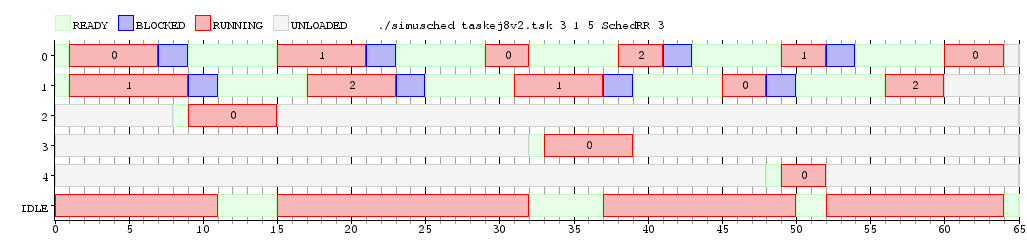
\includegraphics[width=1\textwidth]
   	 {imgs/8Migracion2.png}
	\caption{Situación desfavorable con migración. Q = 3, N = 3, Tmigracion = 5.}
\end{figure}


\begin{figure}[H]
  	\centering
   	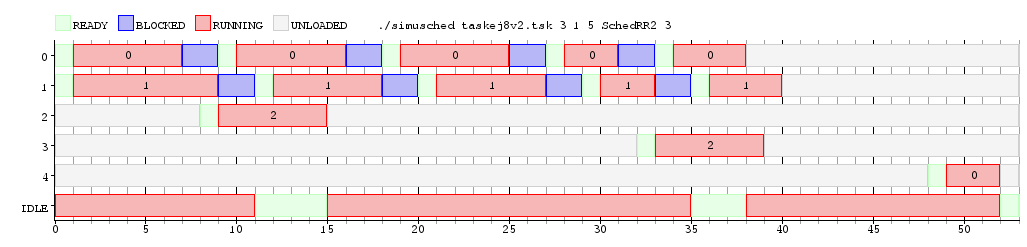
\includegraphics[width=1\textwidth]
   	 {imgs/8NoMigracion2.png}
	\caption{Situación favorable sin migración. Q = 3, N=3.}
\end{figure}

En este ejemplo,se ilustra un caso que desfavorece a la migración de núcleos. Notemos que existe una penalidad de tiempo(costo de migración)que se suma cada vez que
un proceso cambia de núcleo. Al igual que el tiempo de cambio de tarea(context switch), es un intervalo en el que el cpu no hace ningún trabajo "útil" para algún proceso.
La situación que se plantea, en este caso , muestra que el intercambio constante de núcleos, para un proceso, puede terminar siendo desventajoso.
Básicamente, hay dos tareas, que se bloquean alternadamente con cierto desfase, con una duración mayor a las ultimas tres . Se da que cada que cuando la tarea de \textbf{id0} se encuentra  bloqueada, llega una nueva tarea \textbf{TaskCpu}. En ese instante, se le asignará siempre  el primer núcleo disponible(que es el cero, porque la tarea que estaba ejecutando se bloqueó).
Esto provocará que entonces, cuando la primera retome la ejecución lo haga en el  núcleo 1(pues el cero seguirá ocupado) y por esta misma razón, cuando la segunda vuelva a su estado de  "ready" solo podrá tomar el núcleo 2(porque aun las otras tienen tomado los demás cores). Esta particularidad forzó que las dos primeras tareas migraran sus núcleos, pero no trajo ningún beneficio ,si no lo contrario. De esta manera, iran llegando otras dos tareas que surtan el mismo efecto sobre las dos primeras, las de \textbf{id0 y id1}.

Si se actúa sin migración, se da lo que uno esperaría en un principio. Cuando llega una tarea corta, como hay un núcleo disponible y las taras de \textbf{id1 y id2} están fijas en la cola de tareas del núcleo cero y uno respectivamente, se le otorga el core restante(el dos). Esto "paralelizara" las tareas de una forma mas eficiente, decrementando el \textbf{waiting time y running time}.



\textit{Nota(Throughput): Cuanto mas alto, mejor.}




\subsection{Resolución:}

Para implementar este Round Robin, que no tiene migración entre núcleos, se usaron tres arreglos de enteros, un arreglo de colas, un vector de tuplas y un entero. Los arreglos de enteros, que todos tienen el tamaño de la cantidad de cores, son : \textbf{contadores}, que va a tener cuanto corrió una tarea en cada core, \textbf{quantum}, que va a tener el quantum de cada core, y \textbf{CantBloq}, que en un principio va a tener todas las posiciones en cero. El arreglo de colas va a tener una cola por cada core. El vector de tuplas va a aguardar en que core va a ir una tarea cuando se desbloque. El entero es para saber la cantidad de cores que hay.

En un principio cuando empieza el programa inicializa todas las estructuras y espera con la tarea idle. Cuando llega una tarea nueva nos fijamos cuál de todos los cores tiene la menor cantidad de tareas (ya sea corriendo, en espera o bloqueadas) y la encolamos en la cola que corresponde a ese core. Cuando empieza a correr la tarea se pone en cero la posición que le corresponde al core en el arreglo \textbf{contadores}. En cada tick del reloj se va a aumentar en uno una posición  del arreglo \textbf{contadores}, según el core, y nos fijamos en esa misma posición pero en el arreglo \textbf{quantum} para ver si la tarea tiene que ser desalojada o no, y en el caso de tener que hacerlo devolvemos la tarea a la cola que le corresponda y desencolamos la próxima, volviendo a poner a en esa posición de \textbf{contadores} el valor cero.

En caso de que una tarea se bloque se aumenta en uno a la posición que le corresponde al core en el que corre la tarea en el arreglo "CantBloq", y se crea una tupla en la que guardamos el pid y el core que le corresponde a la tarea bloqueada y lo agregamos al final del vector de tuplas. Luego nos fijamos si hay otra tarea para correr y en caso de que no lo haya corre la tarea idle. Cuando se desbloque la tarea se busca en el vector de tuplas la tupla que tiene el pid que se desbloqueó para saber a qué cola agregarla, y sacamos esa tupla del vector, también decrementamos en uno "CantBloq" en la posición correspondiente.


\end{document}

	
